\chapter{Vertex}
\label{Chapter:Vertex}
Identification of heavy flavour quarks, namely b and c quarks, as well as tau leptons is essentially important for CEPC physics. Hence the precision measurement of short length trajectories and secondary vertices imprinted by short lived particles is necessary. The goals therefore drive the need of a precise and low mass vertex detector.


The CEPC vertex detector, consisting of a central barrel section with three super-layers each comprising two silicon pixel layers, provides very precise measurement of the charged particles' track parameters in the vicinity of the interaction point, and reconstructs vertices combining with other tracking detectors. It is the same geometry as that of ILD detector in the ILC \cite{Behnke_2013}, with some dedicated considerations on pixel sensors specifications.

\section{Performance Requirements and Detector Challenges}

The performance of a vertex detector may be parameterized by the resolution on the impact parameter of charged tracks. For instance, the ILD vertex system assumes a resolution of
$$\sigma_{r\phi}=5um\oplus\frac{10}{p(GeV)sin^{3/2}\theta}$$
which can be translated into specifications of the system. The CEPC vertex detector will have the same vertexing performance as above. In order to reach that, the vertex detector should comply with the following specifications:
\begin{itemize}
	\item A spatial resolution near the IP better than 3 um;
	\item A material budget below 0.15\% X0/layer;
	\item A first layer located at as close to beam pipe as possible;
	\item A pixel occupancy not exceeding 1\%.
\end{itemize}


Not like in ILC, the CEPC detector will operate in continues mode, which leads the power consumption of pixel sensors as low as $50mW/cm^2$, if the air cooling could be used inside the detector sensitive volume. Due to beam time structure, the sensor readout time is required to be 20us or faster.


The required radiation tolerance, both for the total ionising dose and the fluence amount, will be lower than those of ILD, based on the beam related background calculation (see chapter MDI).


\section{Baseline design}
The baseline design of the vertex detector is exactly the same as that of ILD, which consists of three, nearly cylindrical, concentric layers of double-sided ladders, as shown in figure \ref{fig:view}. Each ladder is equipped with pixel sensors on both sides, 2 mm apart, resulting in six measured impact positions for each charged particle traversing the detector. The radii covered by the detector range from 16 mm to 60 mm. The material budget of each ladder amounts to $\leqslant$0.3\% X0, equivalent to 0.15\% X0/layer.
\begin{figure}[h!]
	\centering
	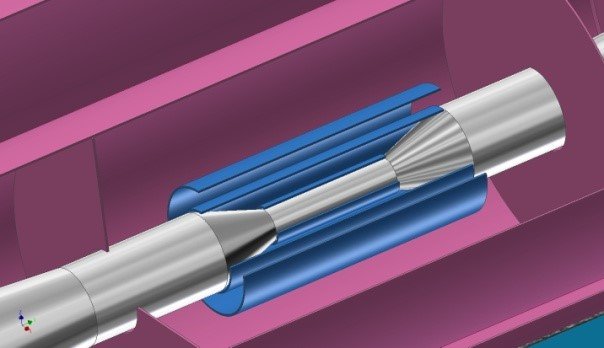
\includegraphics[scale=1.5]{Figures/Vertex/view_of_pixel.jpg}
	\caption{Schematic view of pixel detector (blue)}
	\label{fig:view}
\end{figure}


The layout of the vertex detector is summarized in Table \ref{tab:structure}. It is based on extensive simulation and technical studies from ILD. According to the fast simulation results (see sector 4), the impact parameter resolution can reach the requirement by using the single point resolutions provided in the table.
\begin{table}[!h]
	\centering
	\begin{tabular}{c|c|c|c|c|c}
		\hline
		\ & $R(mm)$ & $\arrowvert z \arrowvert(mm)$ & $\arrowvert cos \theta\arrowvert$ & $\sigma(um)$ & $Readout\ time(us)$\\
		\hline
		Layer 1 & 16 & 62.5 & 0.97 & 2.8 & 20 \\
		\hline
		Layer 2 & 18 & 62.5 & 0.96 & 2.8 & 20 \\
		\hline
		Layer 3 & 37 & 125.0 & 0.96 & 4 & 20 \\
		\hline
		Layer 4 & 39 & 125.0 & 0.95 & 4 & 20 \\
		\hline
		Layer 5 & 58 & 125.0 & 0.91 & 4 & 20 \\
		\hline
		Layer 6 & 60 & 125.0 & 0.90 & 4 & 20 \\
		\hline
	\end{tabular}
	\caption{Vertex detector parameters}
	\label{tab:structure}
\end{table}


\section{Detector performance studies}

The identification of heavy flavor jets through the displaced vertex of longlived beauty and charm hadrons has proven to be a crucial technique in previous experiments. For 240GeV operation charged particles carrying the lifetime information in the jets are often quite soft. Therefore, flavor tagging depends crucially on the precise reconstruction of low momentum (<10GeV) tracks, where multiple scattering dominates the performance. The main performance measure was the impact-parameter resolution projected in the transverse plane sigma(d0), which is closely linked to the flavour-tagging capability of the detectors. The goal is usually expressed in terms of the following parameterization of the transverse impact parameter resolution in a cylindrical vertex detector with uniform spatial resolution and material:
$$\Delta d_{0}[um]=a[um]\oplus\frac{b}{p(GeV)sin^{3/2}\theta},\ where\ the\ design\ value\ of\ ILD\ a = 5,\ b=10.$$


The vertex detector performance has been evaluated for the baseline configuration in full GEANT4 simulations as well as in fast LDT simulations \cite{xx2}. In addition, following the studies of CLIC \cite{dannheim2011layout}, the fast simulation setup was used for geometry optimization studies and to evaluate the sensitivity of the results on the chosen parameters. Assessing the impact of the detector geometries and material budgets on flavor-tagging performance requires dedicated full-simulation studies and will be subject of future R\&D.

\subsection{Performance of the Baseline Configurations}
The impact parameter resolution following from the single point resolutions provided in the table is displayed in figure \ref{fig:angle} as a function of the particle momentum, showing that the ambitious impact parameter resolution is achievable.
\begin{figure}[h!]
	\centering
	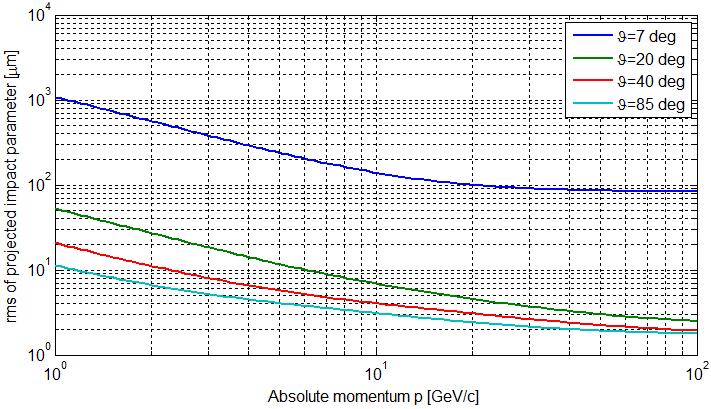
\includegraphics[scale=0.7]{Figures/Vertex/ipr_for_ang.png}
	\caption{Transverse impact-parameter resolutions for single muon events
		as a function of the momentum for different polar angles.}
	\label{fig:angle}
\end{figure}

\subsection{Material Budget}

The baseline designs include very small material budgets for the beam pipe as well as for the sensor layers and their support. To assess the sensitivity of the performance on the amount of material, the material budget for the beam pipe and for the detection layers of the vertex detector has been varied. The resulting transverse impact-parameter resolutions for low-momentum tracks are shown in figure  \ref{fig:material}. When increasing the thickness of the beam pipe by a factor of two, the resolution for tracks at theta= 90 degree increases by approximately 20\%. The same sensitivity is observed for doubling the material in all vertex layers.
\begin{figure}[h!]
	\centering
	\subfigure[] {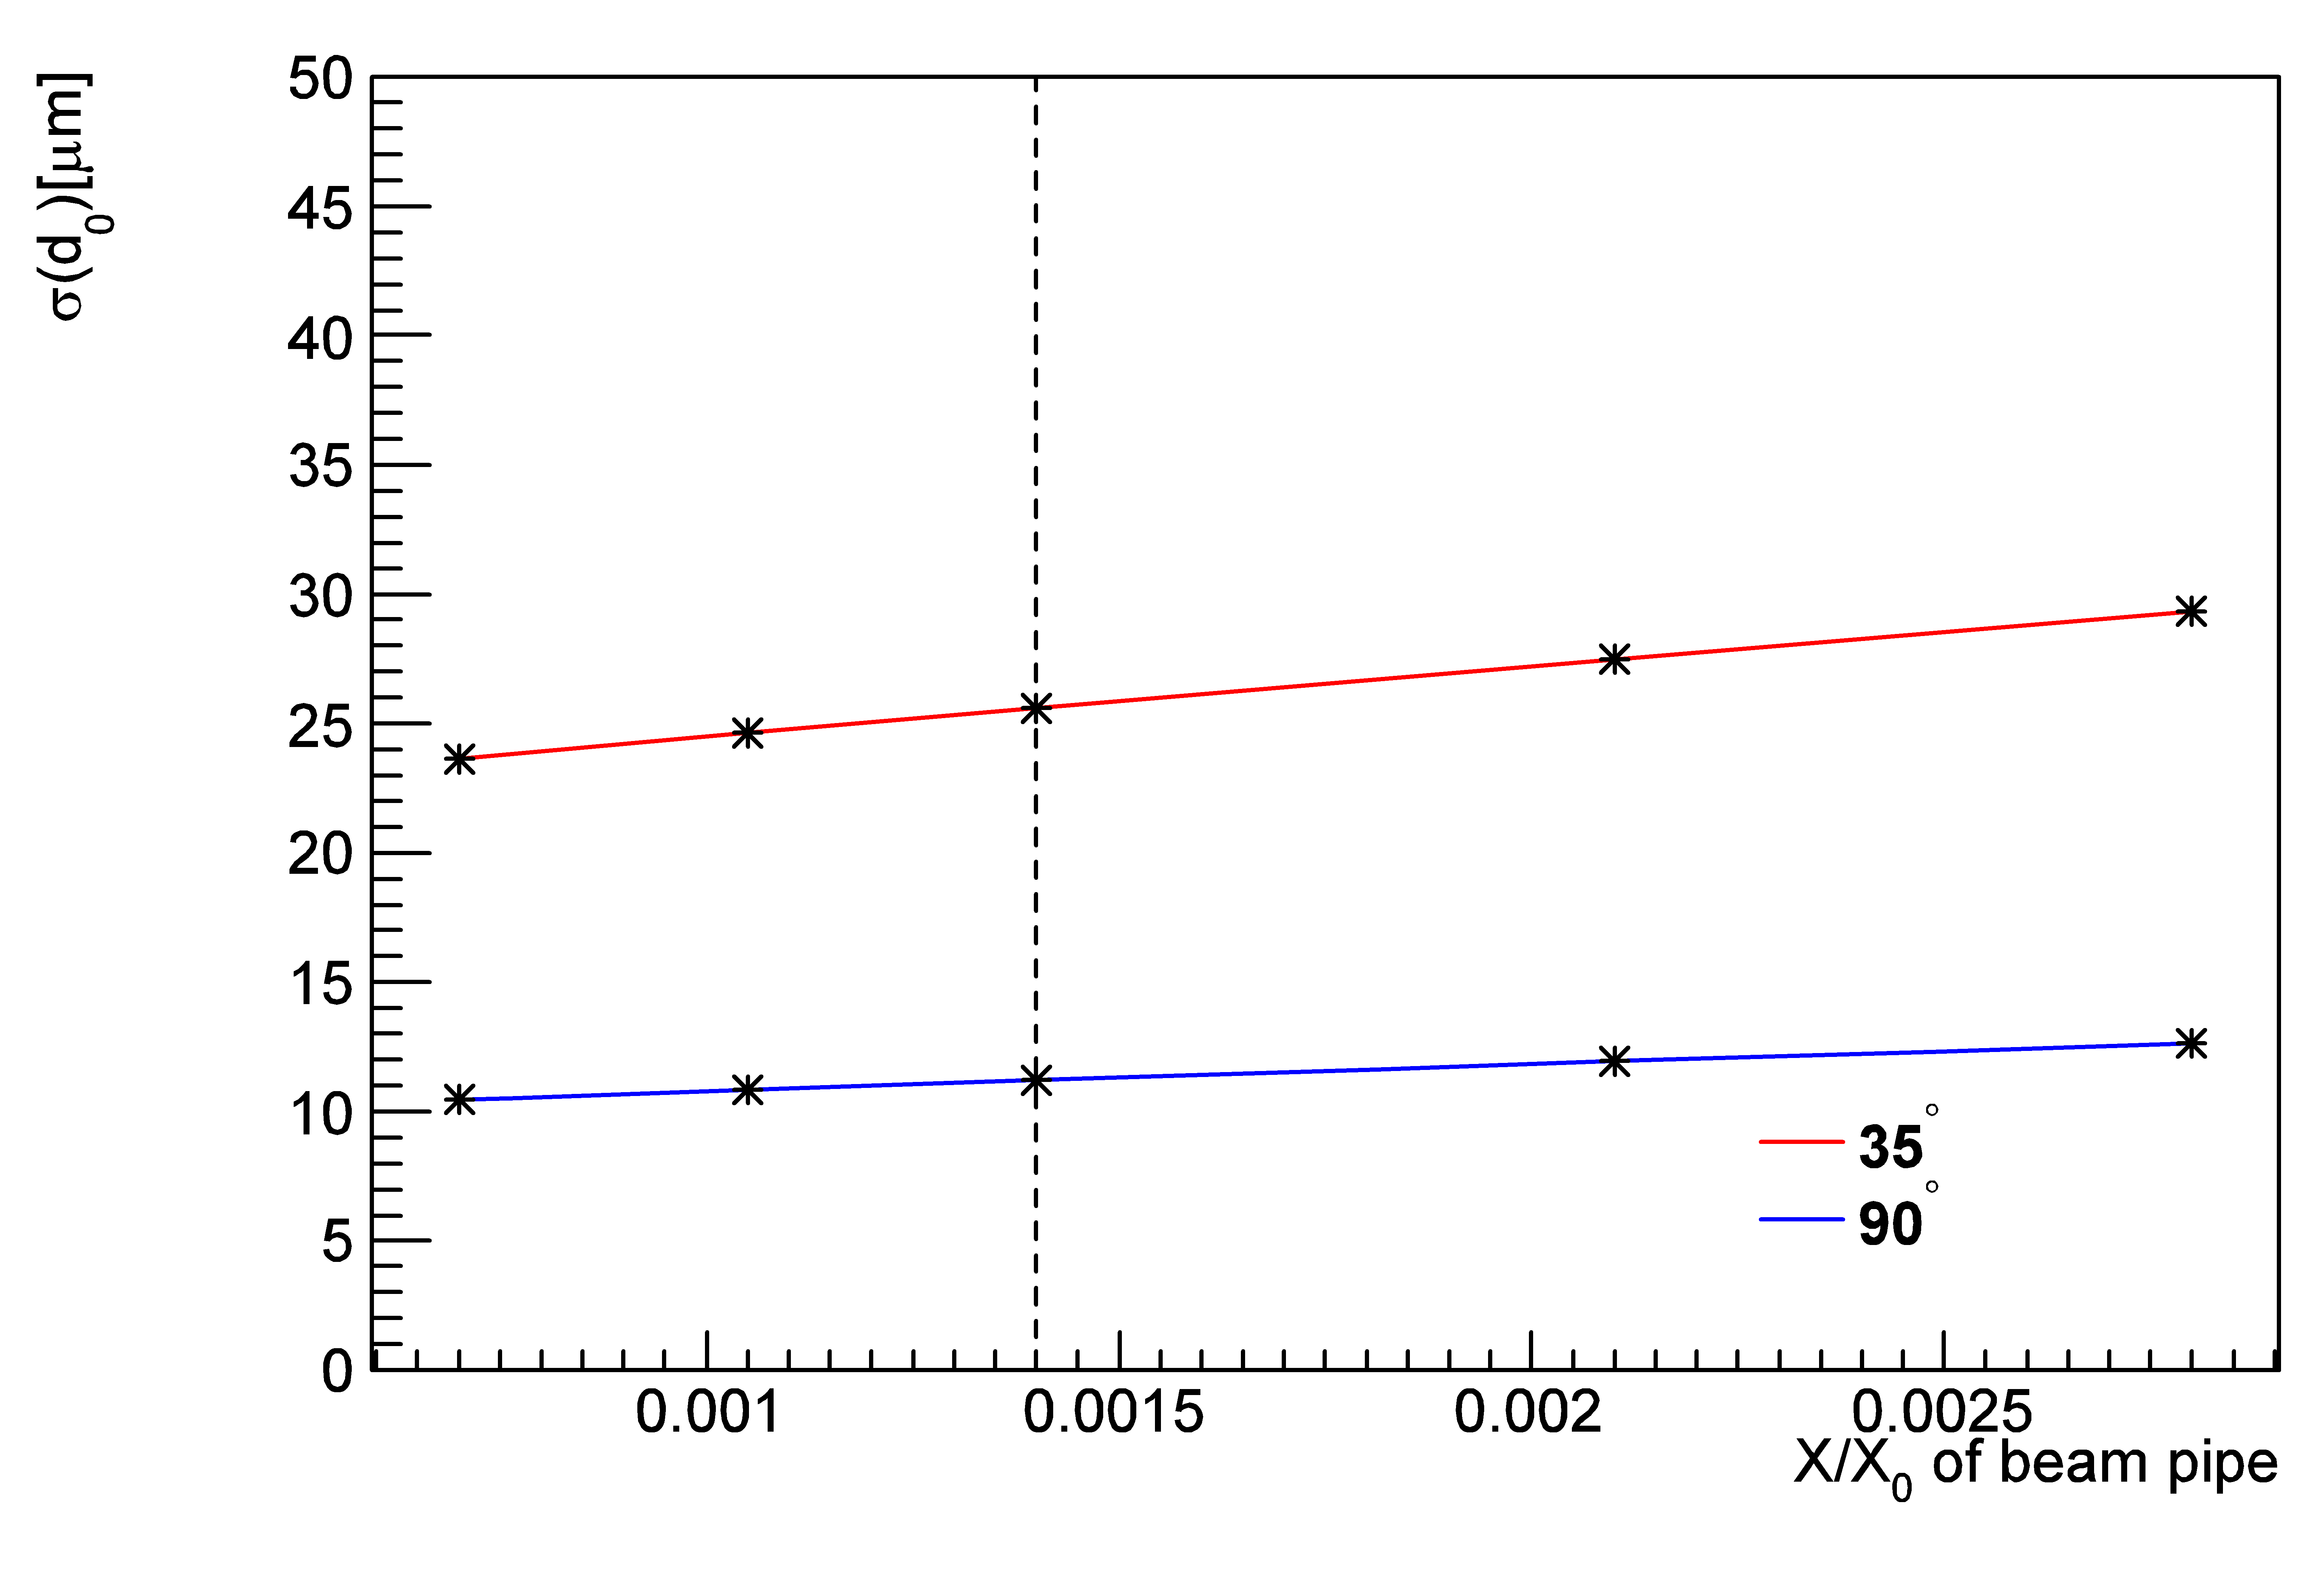
\includegraphics[height=2.2in,width=2.6in,angle=0]{Figures/Vertex/ipr_for_mb_1.png}}
	\subfigure[] {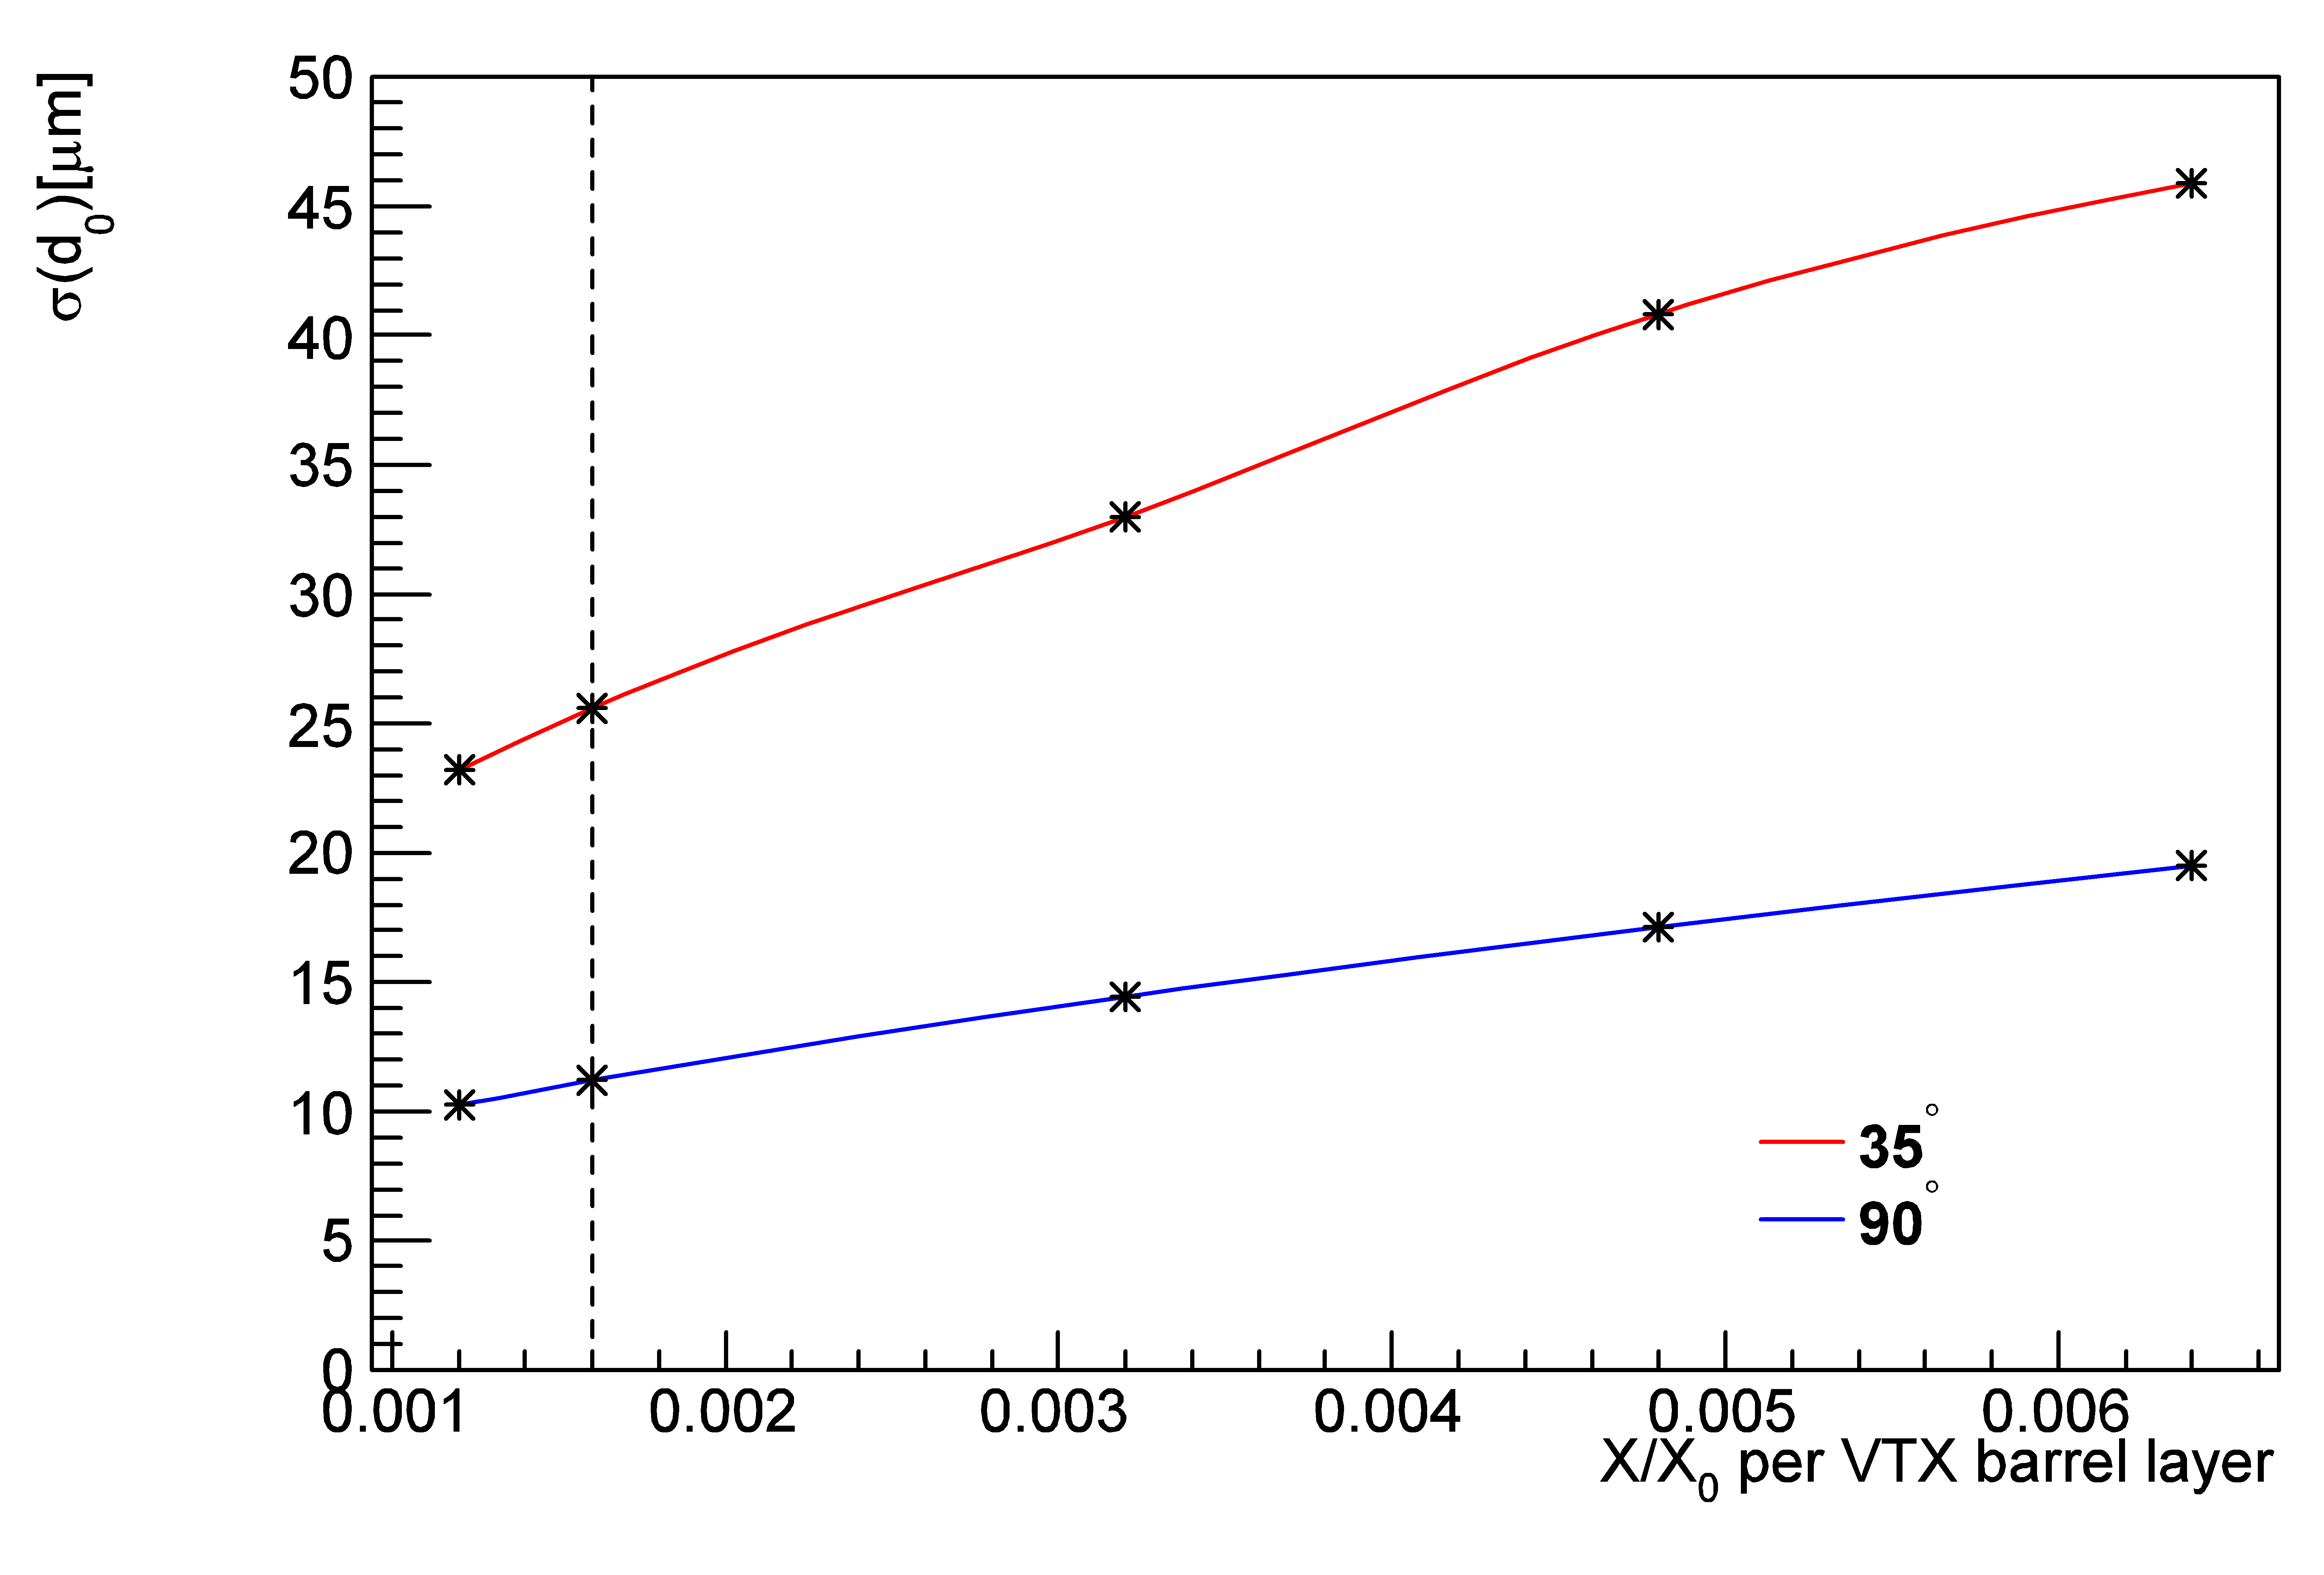
\includegraphics[height=2.2in,width=2.6in,angle=0]{Figures/Vertex/ipr_for_mb_2.png}}
	\caption{Transverse impact-parameter resolution of the CEPC vertex detector as function of the amount of material inside the beam pipe (a) and inside the vertex barrel double layers (b), as obtained from the fast LDT simulation. The results are shown for 1GeV tracks and for polar angles of theta = 35 degrees and of theta = 90 degrees. The material budget corresponding to the baseline configuration is indicated by dashed lines.}
	\label{fig:material}
\end{figure}

\subsection{Dependence on Single-Point Resolution}

The dependence of the transverse impact-parameter resolution on the pixel size was studied by varying the single-point resolution for the simulation of the vertex layers by +50\% w.r.t. the baseline values. The resulting resolutions for high and low track momenta as function of the polar angle theta are shown in figure \ref{fig:res}. The resolution for track momenta of 10GeV is found to change by approximately 30\% larger in the barrel region. Here they exceed the target value for the high-momentum limit of a ~= 5um for both pixel sizes, as expected from the corresponding single-point resolutions. For 1GeV, where multiple-scattering effects dominate, the corresponding variation of the transverse impact-parameter resolution is only 10\% larger. The target value for the multiple-scattering term of b~=10um is approximately reached for both pixel sizes. It should be noted, however, that the pixel size is also constrained by the background occupancies (see chapter MDI) and the ability to separate adjacent tracks in very dense jets in the presence of such backgrounds.
\begin{figure}[h!]
	\centering
	\subfigure[] {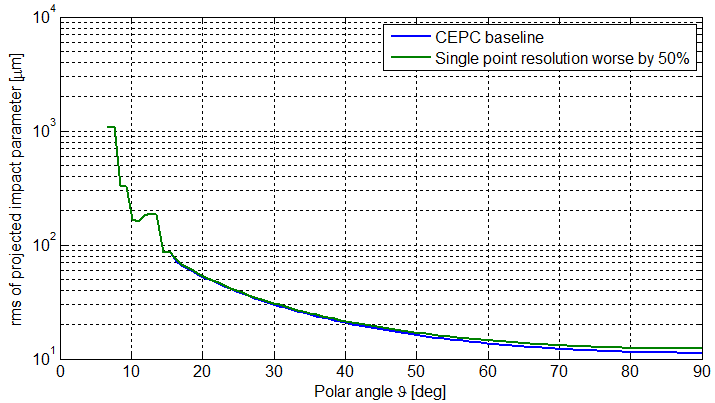
\includegraphics[height=2.2in,width=2.6in,angle=0]{Figures/Vertex/ipr_for_1.png}}
	\subfigure[] {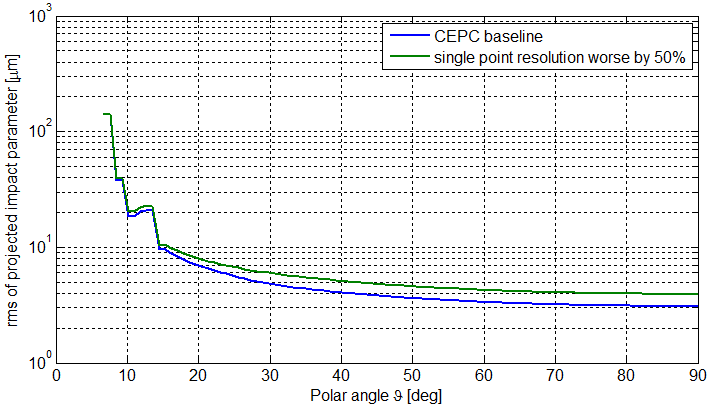
\includegraphics[height=2.2in,width=2.6in,angle=0]{Figures/Vertex/ipr_for_10.png}}
	\caption{Transverse impact-parameter resolution as function of the polar angle theta for different values of the single-point resolution of the CEPC barrel vertex detector, as obtained from the fast LDT simulation. Shown are the resolutions for 1 GeV tracks (a) and for 10 GeV tracks (b).}
	\label{fig:res}
\end{figure}

\subsection{Distance to IP}

The distance of the central beam pipe and barrel vertex layers to the IP was varied by the same amount for all layers of the CEPC vertex detector. Figure \ref{fig:distance} shows the resulting transverse impact-parameter resolutions at theta = 90 degrees as function of the momentum with different radial distance of the innermost barrel vertex layer to the IP. For low momentum tracks, the transverse impact-parameter resolution is proportional to the inner radius.
\begin{figure}[h!]
	\centering
	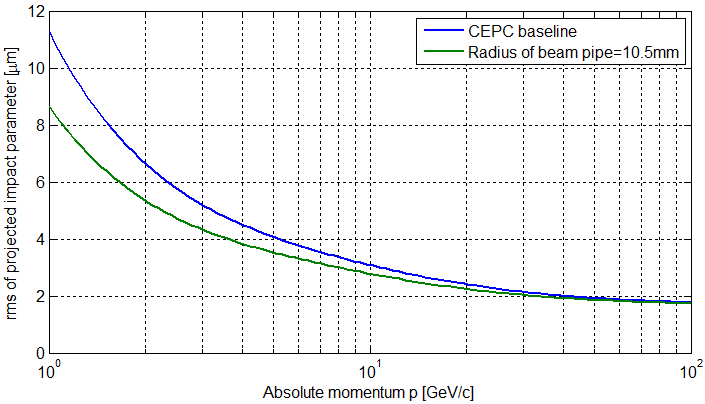
\includegraphics[scale=0.7]{Figures/Vertex/ipr_for_mom.png}
	\caption{Transverse impact-parameter resolution at theta= 90 degrees as a function of the momentum. Blue curve indicates the baseline configuration and the green curve indicates the configuration with the radius of beam pipe=10.5 mm.}
	\label{fig:distance}
\end{figure}

\section{Beam-induced Background in the Vertex Detector}

\section{Sensor Technology Options}

The history of silicon pixel vertex detector could be traced back to LEP era, when it was introduced in the DELPHI experiment \cite{andreazzadelphi}, and significant progress has been made over the last 20 years \cite{hartmann2009delphi}. There have been lots of R\&D efforts towards pixel sensors for vertex tracking in the future particle physics experiments \cite{battaglia2013r}, driven by track density, single point resolution and radiation level. 


As outlined in Section 2, the detector challenges include high IP resolution, low material budget, low occupancy and sufficient radiation tolerance (mild comparing to ILC but not necessarily easy to achieve). To fulfill these requirements of system level, the vertex must be based on sensor technologies which push for fine pitch, low power and fast readout. In the CEPC case it is a unique scenario that might be more requiring than previous applications. In the ILC\cite{Behnke_2013} and CLIC\cite{linssen2012physics}, for example, the power consumption is expected to be significantly reduced by choosing operation of power pulsing, but it is not practical for CEPC. Some other experiments such as the STAR\cite{contin2015maps}, BELLEII\cite{lacasta2014depfet} and ALICE upgrade\cite{abelev2014technical} do their readout continuously the same way the CEPC does. However, they require less in terms of IP resolution and material budget. A sensor technology that fits perfectly in needs of the CEPC does not exist. A few options are listed here for being either close to it or having outstanding potential.


The DEPFET has a unique feature that the main heat sources are located at the end of staves. As the thermal simulation of the BELLEII staves shown in figure \ref{fig:thermal}, 1W for sensitive area and another 1W for switcher located within the acceptance can be cooled by a gentle air flow, while the major heat of 16W in total for readout ASICs located out of acceptance can be removed by massive $CO_{2}$ cooling. The half stave for the BELLEII has achieved a low material budget of 0.21\% and a fast readout of 20us/frame. With a sensitive area of 64.4mm*12.5mm, it seems applicable as the inner most layers of the CEPC. A rough estimate results in 2.5W/ladder in sensitive area and 50us/frame readout speed due to finer pixel pitch required by the CEPC. It needs further investigation As the largest possible size of a half stave is limited to be inside a 6-inch wafer, the length of outer layers gets out of reach for the DEPFET.
\begin{figure}[h!]
	\centering
	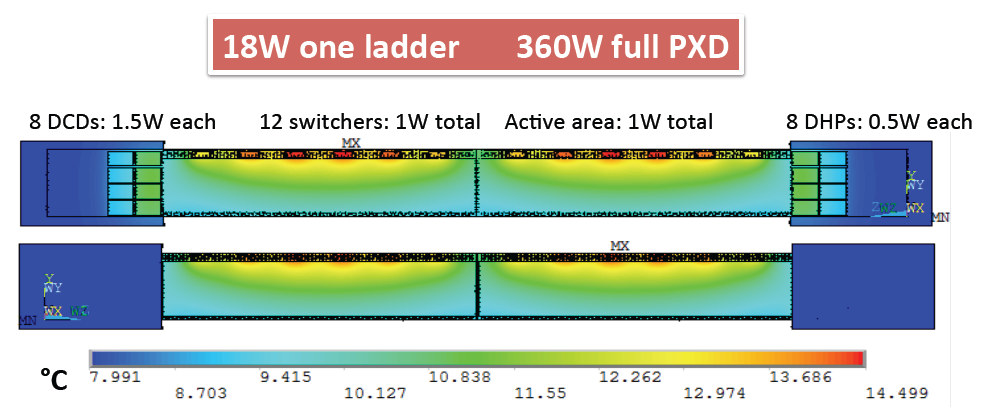
\includegraphics[scale=0.5]{Figures/Vertex/thermal_simu.png}
	\caption{Thermal simulation of the BELLEII staves}
	\label{fig:thermal}
\end{figure}


The HR-CMOS is gaining momentum from R\&Ds for the ALICE upgrade. Considering success of the MAPS (its predecessor) in the STAR and rapid progress achieved in the ALICE upgrade, HR-CMOS is possibly the most mature technology for an application like the CEPC. It has been approved to meet every single aspect of requirements of a CEPC-like detector. However, it is still challenging as to put all the specifications into a single chip. Intensive studies on circuit optimization (in-pixel discrimination) and innovative readout scheme (column sparsification) are underway. Pushing the power consumption down to $50mW/cm^2$ is a critical goal for application in the CEPC case.


The SOI is an option with great potential. The issue of coupling between sensor and circuit has been well understood and is addressed properly. There are a wide variety of applications in astrophysics\cite{nakashima2013development}, material science\cite{hatsui2013direct} and particle physics\cite{ONO2013266} which keep the MPW running steadily. This technology features fully depleted high resistive substrate, 0.2um full CMOS process and being apt to 3D integration. The IHEP group has been developing both chips with fine pitch and chips with complicated function for over 3 years. Making best use of the high quality sensor and the SOI CMOS process could lead to good S/N ratio, which benefits an optimum solution of low power and fast readout. Similar to the HR-CMOS, the upper limit of power consumption is set to 50mW/cm2.


The criteria of being able to cope with continuous colliding and to still remain low power distinguished the 3 sensor options out of other technologies on market. Both the Chronopixel proposed for SiD/ILC and the CLICpix for the CLIC, for example, consume large amount of current in pixel level and rely on power pulsing heavily. HV-CMOS\cite{peric2012active} is proposed more like a hybrid sensor and only minimum electronics on chip. The current R\&D efforts are focusing on ATLAS-alike architectures and are definitely not suitable for precise measurement on an electron-positron collider.

\section{Mechanics and Integration}

The design of the vertex detector is conceived as a barrel structure, including six concentric layers. The preliminary layout of each layer is shown in table \ref{tab:layout}. The range of the radii covered by the detector is from 16mm to 60mm. The length of layers 3 to 6 is 125cm, which is twice as long as the first two layers.
\begin{table}[!h]
	\centering
	\begin{tabular}{c c c}
		\hline
		No. of layer & radius (mm) & length (cm) \\
		\hline
		Layer 1 & 16 & 62.5 \\
		\hline
		Layer 2 & 18 & 62.5 \\
		\hline
		Layer 3 & 37 & 125.0 \\
		\hline
		Layer 4 & 39 & 125.0 \\
		\hline
		Layer 5 & 58 & 125.0 \\
		\hline
		Layer 6 & 60 & 125.0 \\
		\hline
	\end{tabular}
	\caption{The preliminary layout of each layer}
	\label{tab:layout}
\end{table}


The detector may be realized by 3 double-sided layers. Each double-sided layer is equipped with pixel chips on both sides, and has a common support frame. In the azimuthal direction, each layer is segmented in elements called ladders. The ladder, which extends over the whole length of the layer, is the basic building block of the detector. It contains all structural and functional components, such as chips, flex cable, support frame and cold plate if it is necessary. Pixel chips in a row are connected to flex cable by wire bonding or other bonding techniques, and then glued to the support frame, which is composed of low Z materials, such as carbon fiber and silicon carbide, providing stable mechanical support. The other side of the support frame is equipped with another pixel chips layer. 


The design of the ladders should take into account the specifications of the vertex detector. In order to reduce a small multiple Coulomb scattering contribution to the charged-track vertex resolution and control deformations from gravity and cooling forces for the sensors position stability, the ladder mechanical support must fulfill stringent requirements in terms of minimum material budget and highest stiffness. The ladder design of other experiments can be as references, such as STAR pixel detector (PXL), the upgrade of ALICE inner tracking system (ITS) and BELLEII pixel detector (PXD), especially ILD vertex system, which takes double-sided ladder as an alternative ladder design. 


The ladder mechanical support is inherently linked to the layout of the cooling system that will be adopted to remove the heat dissipated by the pixel sensors since the cooling system is integrated in the mechanical structure. The key point of the cooling system design of the vertex detector must balance the conflicting demands of efficient heat dissipation with a minimal material budget. So suitable cold plate, which is coupled with pixel sensors, with high thermal conductivity and low material budget should be taken into account in the ladder design. There are two main types of cooling methods in particle physics experiments, air cooling and active cooling. Table \ref{tab:cooling} gives a list of cooling methods and the corresponding material budget of each layer of the aforementioned experiments. The upgrade of ALICE ITS \cite{abelev2014technical} adopts water cooling with respect to a chips power dissipation value of 300mW/cm2. Polyimide cooling pipes fully filled with water are embedded in the cold plate. STAR- PXL \cite{wieman2009star} uses air cooling according to its chips power consumption of $170mW/cm^{2}$. For ILD \cite{Behnke_2013} vertex system, two different cooling options are considered, depending on the sensor technology. The sensors and SWITCHER chips of BELLE II PXD \cite{abeoctober} require air cooling, while active cooling will be used for readout chips on each end of the detector, which is out of the sensitive region of the detector. So for CEPC vertex detector, the suitable cooling method will be determined according to the sensor option and the power consumption.
\begin{table}[!h]
	\centering
	\begin{tabular}{c c c c}
		\hline
		Vertex detector & Power dissipation & Cooling method & Material budget \\
		& & & requirement/layer \\
		\hline
		Alice ITS & $300\ mW/cm^2$ & water & 0.3\% \\
		\hline
		STAR PXL & $170\ mW/cm^2$ & air &  0.39\% \\
		\hline
		ILD vertex & <$120 mW/cm^2$ (CPS and DEPFEET) & air or $N_2$ & 0.15\% \\
		& 35W inside cryostat (FPCCD) & two-phase $CO_2$ & \\
		\hline
		BELLEII PXD & 20W for sensor and SWITCHER & Air & 0.2\% \\
		& 180W on each end & $CO_2$ & \\
		\hline
	\end{tabular}
	\caption{Cooling method of the vertex detector in each experiment}
	\label{tab:cooling}
\end{table}


Simulation and module prototype studies should be carried out to find suitable designs that can meet requirements of stability, cooling and the performance of the vertex detector. 


For the design of the whole mechanical structure of the vertex detector, some criteria must be taken into account. Firstly, minimum material has to be used in the sensitive region to reduce multiple Coulomb scattering. Secondly, to ensure high accuracy in the relative position of the detector sensors and provide an accurate position of the detector with respect to the central tracker of TPC and the beam pipe, a mechanical connector or locating pin at each end of the ladder should be considered to allow the fixation and alignment of the ladder itself on the end rings. Thirdly, cooling system should be arranged reasonably to ensure stable heat dissipation. At last, to reduce the dead region caused by the boundary of each ladder, neighboring ladders should be partially superimposed. 


In addition, the main mechanical support structures of the vertex should also meet the requirements of the integration with the other detectors, such as time projection chamber (TPC) and forward tracking disks. 


\section{Critical R\&D}

As outlined above, the proposed vertex detector will be based on novel silicon pixel technologies, with low power consumption pixel sensor, and low-mass mechanical structure, to meet the stringent performance requirements of the experiment. Since the technologies are not mature enough at the moment, there still needs critical R\&D efforts to make them available for engineering construction. 

\subsection{Current R\&D activities}
\subsubsection{CMOS Pixel Sensor}
\subsubsection{SOI Pixel Sensor}

\subsection{Future R\&D}

\subsubsection{Pixel sensors with lower power consumption and higher readout speed}

From the view point of circuit design, readout speed and power consumption contradict to each other. However moving column-shared discriminators into individual pixel would benefit readout speed and power reduction simultaneously in a conventional rolling shutter scheme. More efficient readout schemes can be implemented by in-pixel discrimination and column-coding to avoid periodical polling through the entire pixel array. Much of the improvement and optimization at sensor level are related to such circuit design as mentioned above.

\subsubsection{Mechanical design and cooling}

Cooling, mechanical support and cabling within the acceptance are engineering challenges. In order to build ladders with discrete chips of HR-CMOS or SOI, light weight mechanical support and cabling are necessary with a material budget of less than 0.05\%/X0 each. As for DEPFET all-silicon staves, the total material budget is expected to be 0.15\%/X0. Manufacturing and assembling of those ladders/staves have to be verified. In addition, the vibration must be characterized carefully so as to obtain enough cooling capability and not degrade the IP resolution. In the case of DEPFET, additional $CO_{2}$ cooling has to be introduced to cool the hot spots of ASIC chips, which makes the system more complex.

\subsubsection{Sensor thinning}

Thinning sensors down to 50um has been demonstrated on MAPS chips/wafers, which does not require further process on the backside of chips/wafers. While both DEPFET and SOI require backside process after thinning. DEPFET for BELLEII was thinned to 75um in the sensitive area \cite{lacasta2014depfet} and is likely thinned to 50um without fundamental difficulty. SOI already achieved 110μm thickness without any adverse effect observed  \cite{xx18}. The reliability and yield after thinning to 50um have to be studied carefully.

\section{Summary}

The basic concepts in the ILD Vertex detector, including the pixel sensors' specifications required by IP resolution and radiation tolerance, the low-mass mechanical design, and the barrel geometry, are essentially adapted to the baseline design of CEPC Vertex detector. However, due to CEPC's continuous working mode, the R\&D is critically needed to reduce the sensor power consumption and charge collection time. Further, more detailed designs for mechanical supports and cooling, cabling, and power conversion are also necessary. Most of those issues could be learnt and improved from R\&D activities for the ILC detectors. 




\bibliographystyle{Style/atlasnote} %% plain.bst
\bibliography{Chapters/Vertex} %% bsample.bib

